\chapter{Word-level Traversal of Finite State Machines using Algebraic Geometry}
\label{ch:reacha}
Reachability analysis is a basic component of sequential circuit verification, esp. for 
formal equivalence checking and model checking techniques. Concretely, in modern synthesis 
tools, in order to improve various performance indicators such as latency, clock skew or power
density, some major refactoring and attachments are made on original designs. 
Those modifications may introduce malfunctions or glitches to the whole logic. 
In localized simulation or formal verification (esp. equivalence checking), the modifications may be 
denied since the malfunctions or glitches are considered as ``faults" in this circuit.
However, if the circuit behavior is carefully investigated, it may come to a verdict that 
those ``faults" will never be activated/excitated during a restricted execution starting 
from legal initial states and with legal inputs. Thus we will call those ``faults" as 
{\bf spurious faults}, since they will not affect the circuit's normal behavior.

Almost all practical sequential logic components can be modeled as finite state machines (FSMs). 
If we apply constrains upon the machine to make it start from designated initial states and 
take in specific legal inputs, a set of reachable states can be derived. 
As long as the ``faults" can be modeled as ``bad states", we can judge whether they are 
spurious faults by checking if they sit in the reachable states. From the spurious fault validation 
perspective, reachability analysis is a must when developing full set of sequential circuit verification
techniques.

There are quite a few methods to perform reachability checking on FSMs. One among them is 
state space traversal. Conventionally the algorithm is based on bit-level techniques such as
binary decision diagrams (BDDs) and Boolean logic. We propose a new traversal algorithm on word-level,
which bring critical advantages. In this chapter the approach will be described and discussed in depth, 
with examples and experiments showing its feasibility when applied on general circuit benchmarks.

\section{Motivation}
\subsection{Limitations of Full Scan Algorithms}
The inspiration of this research mainly comes from a journal paper \cite{KallaPartialScan}. 
In that paper, the author proposed an traversal algorithm using concept ``implicit state enumeration".
Concretely, the algorithm is written as follows:

\begin{algorithm}[H]
\SetAlgoNoLine
\LinesNumbered
 \KwIn{Sequential circuit, number of registers to scan}
 \KwOut{Scan registers listed in decreasing order of their non-controllability}

  $from^0 = reached = S^0$\;
  $i = 0$\;
  \While{TRUE}
  {
  	$i++$\;
	$to^i = $IMAGE$(\Delta,from^{i-1})$\;
	$new^i = to^i \cdot \overline{reached}$\;
	\For{each state variable $r_j$}
	{
		record\_if\_transitions\_present\_or\_missing$(r_j,new^i)$\;
		compute\_degree\_of\_unsettability$(r_j,new^i)$\;
	}
	\If{$new^i == 0$}
	{
		break\;
	}
	$reached = reached + new^i$\;
	$from^i = new^i$\;
  }\
  \tcc{\ \ \ \ \ \ \ \ \ \ \ \ \ \ FSM traversal completed}\
  \For{each state variable $r_j$}
  {
	\If{missing transition for $r_j$}
	{
		scan state variable $r_j$\;
	}
  }
  $illegal\_states = $bdd\_complement$(reached)$\;
  \For{each state variable $r_j$}
  {
	compute\_degree\_of\_unateness$(r_j,illegal\_states)$\;
	non-controllability$(r_j)=$degree\_of\_unsettability$(r_j)+$degree\_of\_unateness$(r_j)$\;
  }
  order state variables in terms of their non-controllabilities;\tcc{\ Sorting}\
  output the required scan registers\;
%\Return{$from_k(R_{final})$}
\caption {SIMPSON: Scan Register Selection using Implicit State Enumeration\cite{KallaPartialScan}}
\label{alg:SIMPSON}
\end{algorithm}
\DecMargin{1em}

Note that the former part of this algorithm describes a breath-first-search (BFS) traversal in
state space. The traversal algorithm is a simple variation of BFS algorithm in graph theory where 
states are nodes and transitions are arcs. Each state is uniquely encoded by a combination
of a set of register data, which is usually represented by a Boolean vector. 

Since a typical sequential circuit usually contains an functionally independent combinational logic
component, the traversal algorithm analyzes the combinational logic and derive the transition 
function for one-step reachability within current time-frame, and extend the result to complete 
execution paths through unrolling. If each state encoding (i.e. exact values in the selected registers) is
explicitly exposed and counted during the unrolling 
procedure, this unrolling is called {\bf explicit unrolling}. In the SIMPSON algorithm, the states cannot be 
directly read in the execution; instead, they are implicitly represented using a conjuction of several 
Boolean formulas. Such techniques differs from explicit unrolling are called {\bf implicit unrolling}.

However, the SIMPSON algorithm proposed by the author is usually not practical. The conjuctions of 
Boolean formulas are stored as BDDs, which is a canonical and convenient structure. Nevertheless, 
the size of BDD is easy to explode when the formulas become too long and too complicated. In the paper,
the author make a compromise between accuracy and cost, and turn to a partial scan technique rather than 
a full scan. In my research work, the aim is to explore a word-level technique which can make a full scan 
available.

\subsection{Word-level Data Flow on Modern Datapaths}

\subsection{Prerequisites of Word-level Techniques}

\section{FSM Reachability using Algebraic Geometry}
\label{sec:reach}
% \subsection{An example illustrating our proposed approach}
We use symbolic state reachability with algebraic
geometry concepts. It is an abstraction based on word operand
definition of datapaths in circuits, and it can be applied
to arbitrary FSMs by bundling a set of bit-level variables together as
one or several word-level variables.  The abstraction polynomial,
encoding the reachable state space of the FSM, is obtained through
computing a GB over $\Fkk$ of the polynomials of the circuit using an
elimination term order based on Theorem \ref{thm:elim}.  

Conceptually, the state-space of a FSM is traversed in a breadth-first
manner, as shown in Algorithm \ref{alg:BFS}. % \cite{KallaPartialScan}: 
The algorithm operates on the FSM $\mathcal{M} = (\sum, O, S, S^0,
\Delta, \Lambda)$ underlying a sequential circuit. In such cases, the
transition function $\Delta$ and the initial states are represented
and manipulated using Boolean representations such as BDDs or SAT
solvers. The variables $from, reached, to, new$ represent
characteristic functions of sets of states. Starting from the initial
state $from^i = S^0$, the algorithm computes the states reachable in
1-step from $from^i$ in each iteration. In line 4 of algorithm
\ref{alg:BFS}, the {\it image computation} is 
used to compute the reachable states in every execution step. 

The {\it transition function} $\Delta$ is given by Boolean equations
  of the flip-flops of the circuit: $t_i = \Delta_i(s, x)$, where
  $t_i$ is a next state variable, $s$ represents the present   state
  variables and $x$ represents the input variables. The {\it
    transition relation of the FSM} is then represented as:  
\begin{equation} 
T(s, x, t) =   \prod_{i=1}^{n} (t_i \overline{\oplus } \Delta_i)
\end{equation}
where $n$ is the number of flip flops, and $\overline{\oplus}$ is XNOR
operation. Let $from$ denote the set of initial states, then the
image of the initial states, under the transition function $\Delta$ is
finally computed as:
\begin{align}
\label{img}
to = \text{Img}(\Delta, from) = \exists _s ~\exists _x ~[ T(s, x, t)
  \cdot from ] 
%= \exists _s ~\exists _x ~\prod_{i=1}^{n} (t_i \overline{\oplus } \Delta_i)\cdot from
\end{align}

Here, $\exists x (f)$ represents the {\it existential quantification
  of $f$ w.r.t. variable $x$}.  


\IncMargin{1em}
\begin{algorithm}[hbt]
\SetAlgoNoLine
\Indm
 \KwIn{Transition functions $\Delta$, initial state $S^0$}
\Indp

  $from^0 = reached = S^0$\;
  \Repeat{$new^i == 0$}
  {
  	$i \gets i + 1$\;
	$to^i \gets$Img$(\Delta, from^{i-1})$\;
	$new^i \gets to^i \cap \overline{reached}$\;
  	$reached \gets reached \cup new^i$\;
	$from^i \gets new^i$\;
  }
\Return{$reached$}
\caption {BFS Traversal for FSM Reachability}\label{alg:BFS}
\end{algorithm}
\DecMargin{1em}


Let us describe the application of the algorithm on the  FSM circuit
of Fig. \ref{fig:fsm}. {\it We will first describe its operation at the
Boolean level, and then describe how this algorithm can be implemented
using algebraic geometry at word level.} 

\begin{figure}[H]
\centering{
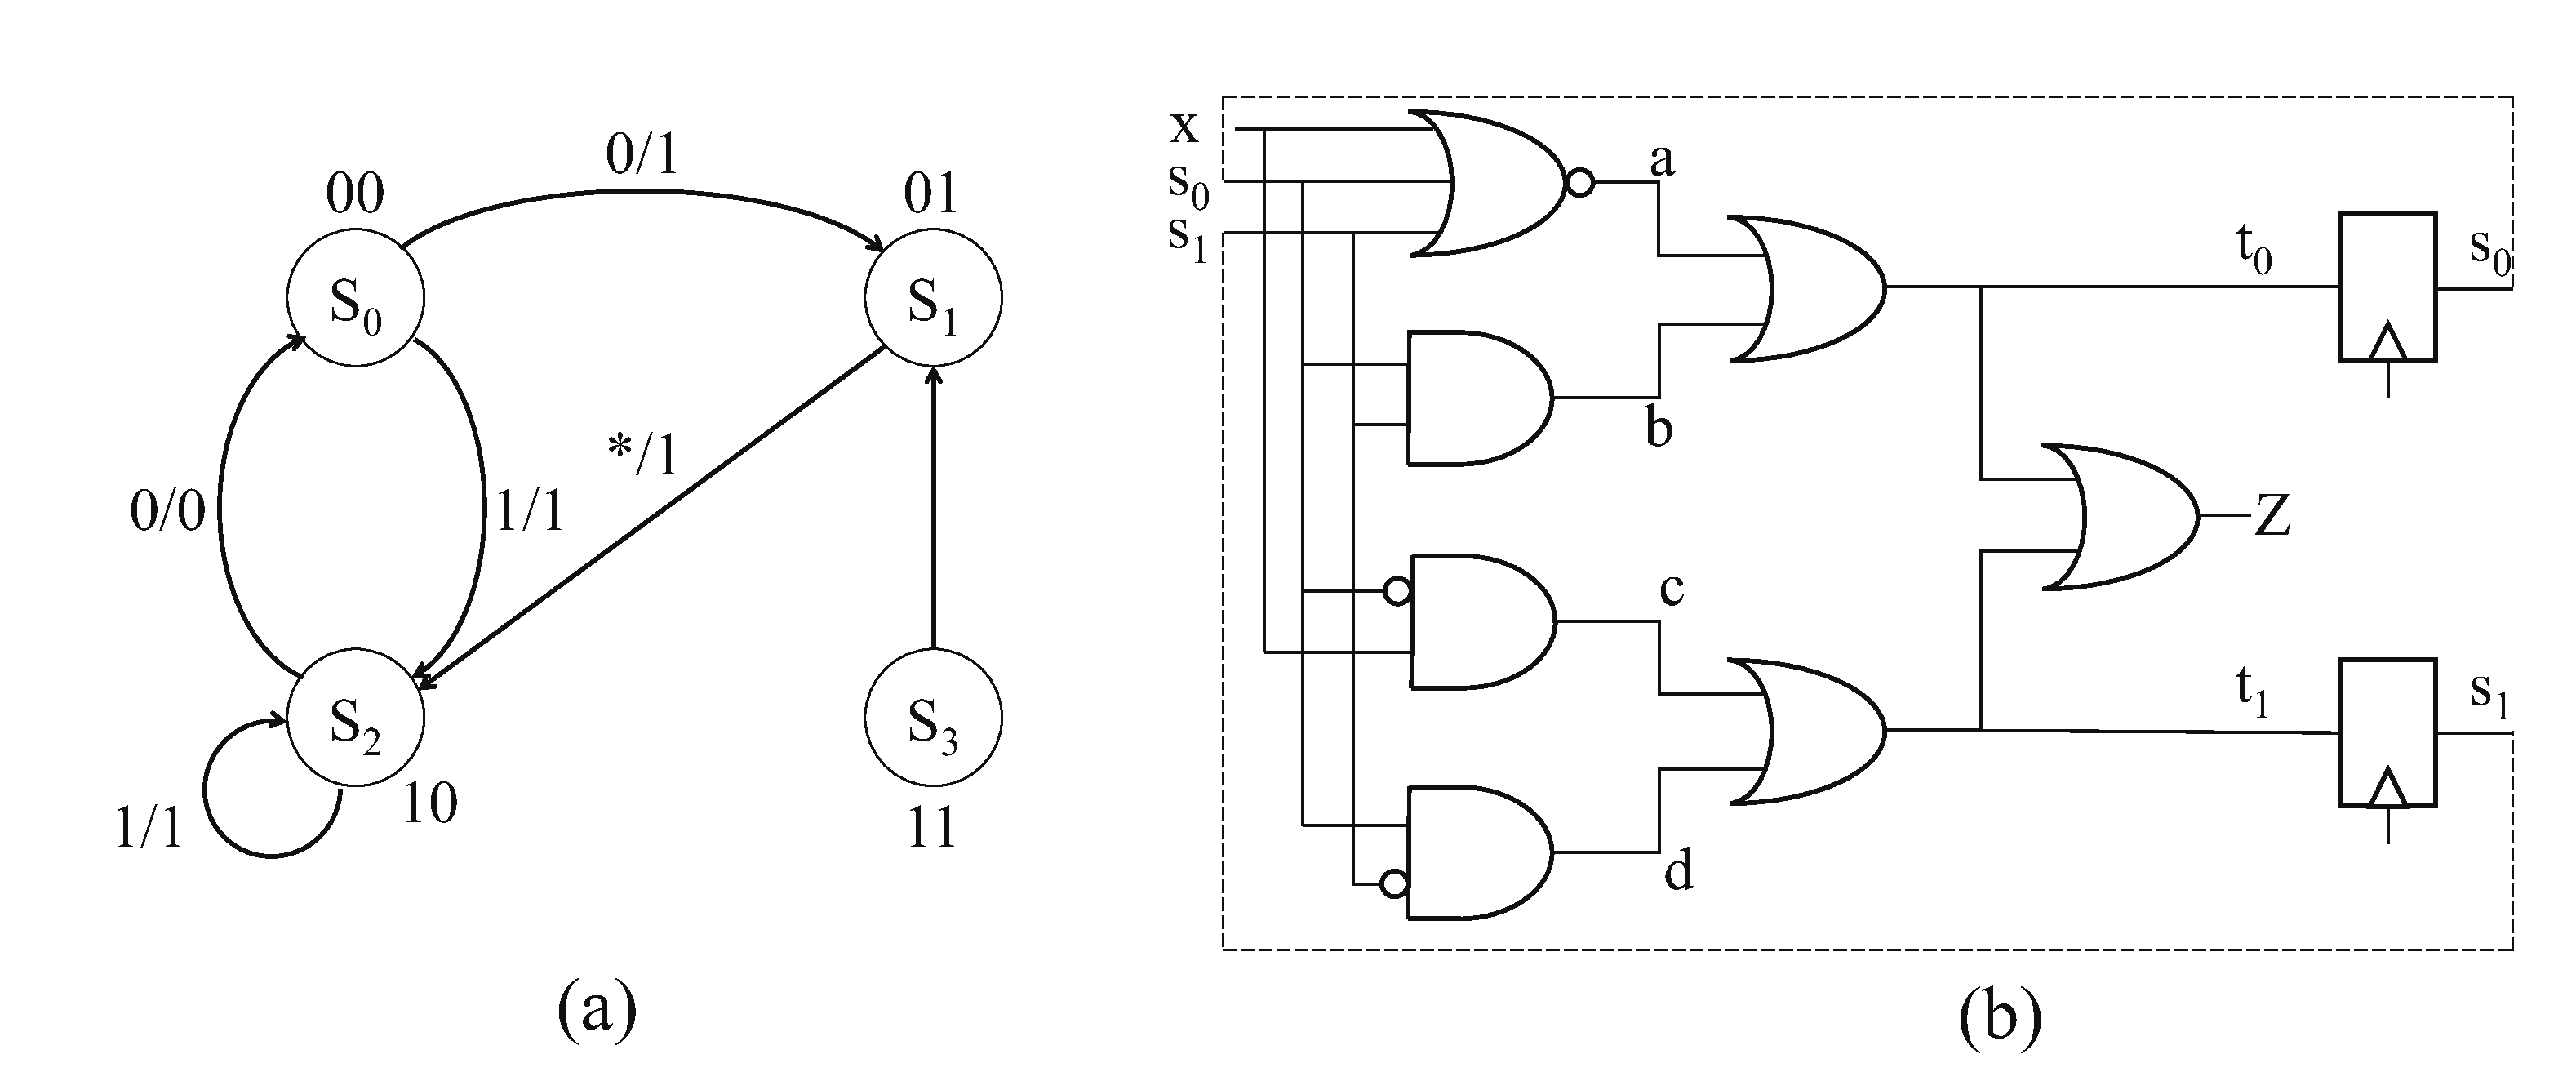
\includegraphics[width=\textwidth]{newfig/new_stg.eps}
\caption{The example FSM and the gate-level implementation. }
\label{fig:fsm}}
\end{figure}

In Line 1 of the BFS algorithm, assume that the initial state
is $S_3$ in Fig.\ref{fig:fsm}(b), which is encoded as 
$S_3 = \{11\}$. Using Boolean variables $s_0, s_1$ for the present
states, $from^0 = s_0\cdot s_1$ is represented as a Boolean formula. 



\begin{Example}
For the circuit in Fig. \ref{fig:fsm} (b), we have the transition
functions of the machine as:

\begin{align*}
\Delta_1: & ~t_0 \overline{\oplus} ((\overline{x \vee s_0 \vee s_1}) \vee s_0 s_1)\\
\Delta_2: & ~t_0 \overline{\oplus} (\overline{s_0}x \vee \overline{s_1}s_0)\\
from:     & ~from^0 = s_0\cdot s_1
\end{align*}

When the formula of Eqn. (\ref{img}) is applied to compute 1-step
reachability, $to = \exists _{s_0, s_1, x} (\Delta_1 \cdot \Delta_2
\cdot from^0)$, we obtain $to = \overline{t_0}\cdot t_1$, which denotes
the state $S_1 = \{01\}$ reached in 1-step from $S_3$.
In the next iteration, the algorithm uses state $S_1 = \{01\}$ as the
current (initial) state, and computes $S_2 = \{10\} = t_0\cdot
\overline{t_1}$ as the next reachable state, and so on. 
\end{Example}

%% Let  $\Delta_i$ denote the transition function for $i^{th}$ bit of the
%% output $T$
%% (denoted by $t_i$), and it is described by a Boolean function. We can
%% obtain the transition relation  for bit-vector $T$:
%% $Tran(s_0,s_1,x,t_0,t_1) =
%% \bigwedge_{i=1}^{2}(t_i\ \bar{\oplus}\ \Delta_i)$. Assume present
%% states are represent by Boolean formulas $PS(s_0,s_1)$, then the image
%% function is written as $\text{Img}(Tran,\ PS) =
%% \exists_{s_0,s_1}\exists_{x}[Tran(s_0,s_1,x,t_0,t_1)\land
%%   PS(s_0,s_1)]$, where $\exists_x f$ denotes the existential
%% quantification of $f$ w.r.t. $x$. 

Our objective is to model the transition functions $\Delta$ as a
polynomial ideal $J$, and to perform the image computations 
%(Algorithm \ref{alg:BFS}, line 4) 
using Gr\"obner bases over Galois fields. {\it
This requires to perform quantifier elimination; which can be
accomplished using the GB computation over $\Fkk$ using elimination
ideals} \cite{gao:qe-gf-gb}. Finally, the set union, intersection and
complement operations are also to be implemented in algebraic geometry.

{\bf FSM Traversal at word-level over $\Fkk$:} 
The state transition graph (STG) shown in Fig.\ref{fig:fsm}(a) uses a
2-bit Boolean vector to represent 4 states $\{S_0, S_1, S_2,
S_3\}$. We map these states to elements in $\mathbb{F}_{2^2}$, where
$S_0 = 0, S_1 = 1, S_2 = \alpha, S_3 = \alpha+1$. Here, we take 
$P(X) = X^2+X+1$ as the irreducible polynomial to construct
$\mathbb{F}_4$, and $P(\alpha) = 0$ so that $\alpha^2 + \alpha + 1 =
0$.  

{\it Initial state:} In Line 1 of Alg.\ref{alg:BFS}, the initial state is
specified by means of a corresponding polynomial $f = \mathcal{F}(S) =
S - 1 - \alpha$. Notice that if we consider the ideal generated by the
initial state polynomial, $I = \langle f\rangle$, then its variety
$V(I) = 1+\alpha$ corresponds to the state encoding $S_3 = \{11\} =
1+\alpha$, where a polynomial in word-level variable $S$ encodes the
initial state. 
% with only one generator $f$, its variety
% $V(I) = \{\gamma\ |\ \gamma \in \mathbb{F}_{2^2}, \gamma = 1+\alpha\}$, which equals to $\{1+\alpha\}$, the only
% valid value $S_3$ can take.


%Using theorems from Section \ref{sec:elim}, we implement the image
%function by a GB computation on elimination ideal. Ex.\ref{ex:motiv}
%is an example for our implementation of image function, i.e. one-step
%reachability. 

{\bf Set operations:} In Lines 5 and 6 of
Alg. \ref{alg:BFS}, we need  \textbf{union}, 
\textbf{intersection} and \textbf{complement} of varieties over
$\mathbb{F}_{2^k}$, for which we again use algebraic geometry concepts.

\begin{Definition}
\label{def:sum}
({\bf Sum/Product of Ideals} \cite{ideals:book}) If $I = \langle f_1,
\dots, f_r\rangle$ and $J = \langle g_1, \dots, g_s\rangle$ are
ideals in $R$, then the {\bf sum} of $I$ and $J$ is defined as $I + J
= \langle f_1, \dots, f_r, g_1, \dots, g_s\rangle$. Similarly, the
{\bf product} of $I$ and $J$ is $I \cdot J = \langle
f_ig_j\ |\ 1 \leq i \leq r, 1 \leq j \leq s\rangle$. 
\end{Definition}

%With concepts of ideal sums and products, we can obtain the
%intersection and union of affine varieties as:
\begin{Theorem}
\label{thm:unionintersect}
If $I$ and $J$ are ideals in $R$, then 
${\bf V}(I + J) = {\bf V}(I) \bigcap {\bf V}(J)$ and ${\bf V}(I \cdot
J) = {\bf V}(I) \bigcup {\bf V}(J)$. 
\end{Theorem}


In Line 5 of Alg. \ref{alg:BFS}, we need to compute the complement of a
set of states. Assume that $J$ denotes a polynomial ideal whose
variety $V(J)$ denotes a set of states. We require the computation of
another polynomial ideal $J'$, such that $V(J')=\overline{V(J)}$. We
show that this computation can be performed using the concept of {\bf
  ideal quotient}:  

\begin{Definition}
\label{def:quo}
({\bf Quotient of Ideals}) If $I$ and $J$ are ideals in a ring $R$, then $I:J$ is the set
%  \begin{equation}
  $\{f \in R \ |\ f\cdot g \in I, \forall g \in J\}$ %\nonumber
%  \end{equation}
and is called the {\bf ideal quotient} of $I$ by $J$.
\end{Definition}

%The following example shows a simple ideal quotient operation:
\begin{Example}
In $\Fq[x,y,z]$, ideal $I = \langle xz,yz\rangle$, ideal $J = \langle z\rangle$. Then
\begin{align*}
I:J &= \{f\in\Fq[x,y,z]~|~f\cdot z \in \langle xz,yz\rangle\} \\
&= \{f\in\Fq[x,y,z]~|~f\cdot z = Axz+Byz\}\\
&= \{f\in\Fq[x,y,z]~|~f= Ax+By\}\\
&= \langle x,y\rangle
\end{align*}
\end{Example}

% However, complement of variety cannot be easily dealt by simple arithmetic on polynomial generators.
% For non-trivial cases we can only prove that 
% \begin{Theorem}
% Let $I, J$ be ideals in $\mathbb F[x_1,\dots,x_n]$, then 
% $${\bf V}(I:J) \supset {\bf V}({\bf I}({\bf V}(I) - {\bf V}(J)))$$
% \end{Theorem}
% Fortunately for most hardware verification cases, the form of polynomial generators are restricted.
% A proposition has been proved by \cite{jinpeng} that after adding {\bf vanishing polynomials ideal}
% the new composed ideal implies following corollary:

We can now obtain the complement of a variety through the following
results which are stated and proved below:

\begin{Lemma}
\label{lem:gcd}
Let $f,g\in \Fkk[x]$, then $\langle f:g\rangle = \left\langle\frac{f}{gcd(f,g)}\right\rangle$.
\end{Lemma}

\begin{proof}
Let $d = gcd(f, g)$. So, $f = df_1 , g = dg_1$ with $gcd(f_1 , g_1 ) =
1$. Note that $f_1 = \frac{f}{gcd(f,g)}$.

Take $h \in \langle f : g\rangle$. According to the
Def. \ref{def:quo}, $hg \in \langle f \rangle$, which means $hg = f
\cdot r$ with $r \in \Fkk[x]$. Therefore, $hdg_1 = df_1 r$ and $hg_1 =
f_1 r$. But considering $gcd(g_1 , f_1 ) = 1$ we have the fact that
$f_1$ divides $h$. Hence $h \in \langle f_1\rangle$.

Conversely, let $h \in \langle f_1 \rangle$. Then $h = s \cdot f_1$,
where $s \in \Fkk[x]$. So, $hg = hdg_1 = sf_1 dg_1 = sg_1 f \in 
\langle f \rangle$. Therefore, $h \in \langle f : g\rangle$.
\end{proof}


\begin{Theorem}
\label{thm:quotient}
Let $J$ be an ideal generated by a single univariate polynomial in
variable $x$ over $\Fkk[x]$, and let the vanishing ideal $J_0 = \langle
x^{2^k}-x\rangle$. Then  
$${ V}(J_0:J) = { V}(J_0) - { V}(J),$$ where all the varieties are
considered over the field $\Fkk$. 
\end{Theorem}

\begin{proof}
Since $\Fkk[x]$ is a principal ideal domain, $ J = \langle g\rangle$
for some polynomial $ g \in \Fkk[x]$. Let $d = gcd(g, x^{2^k} -
x)$. So, $g = dg_1 , x^{2^k} - x = df_1$, with $gcd(f_1 , g_1 ) =
1$. Then $J_0 : J = \langle f_1 \rangle$ by Lemma \ref{lem:gcd}. 

Let $x \in V(J_0 ) - V(J)$. From the definition of set
complement, we get $x \in \Fkk$ while $g(x) \neq 0$.  

Since $x^{2^k} = x$, we see that either $d(x) = 0$ or $f_1 (x) =
0$. Considering $g(x) \neq 0$, we can assert that $d(x) \neq 0$. In
conclusion, $f_1 (x) = 0$ and $x \in V(f_1 )$. 

Now let $x \in V(f_1 )$, we get $f_1 (x) = 0$. So, $x^{2^k} - x = 0$
gives $x \in V(J_0) = \Fkk$ which  contains all elements in the
field. 

Now we make an assumption that $x \in V(g)$. Then $g(x) = 0 =
d(x)g_1(x)$ which means either $d(x) = 0$ or $g_1 (x) = 0$. 

If $g_1 (x) = 0$, then since $f_1 (x) = 0$ we get that $f_1 , g_1$
share a root. This contradicts the fact that $gcd(f_1 , g_1 ) = 1$.

On the other hand, if $d(x) = 0$, then since $f_1 (x) = 0$ and
$x^{2^k} - x = df_1$, we get that $x^{2^k} - x$ has a double root. 
But this is impossible since the derivative of $x^{2^k} - x$ is $-1$.

So, $x \notin V(g)$ and this concludes the proof.
\end{proof}

% Let $J_0 = \langle x_1^{2^k} - x_1, \dots, x_n^{2^k} - x_n \rangle$
% denote the ideal of all vanishing polynomials in $\Fkk$. Then, we have
% $V(J_0) = (\Fkk)^{n}$; i.e. the variety of vanishing ideal contains
% all possible valuations of variables, so it constitutes the {\bf
%   universal set}. Subsequently, based on Theorem \ref{thm:quotient},
% the {\bf absolute complement} $V(J')$ of a variety $V(J)$ can be
% computed as: 

Let $x^{2^k}-x$ be a vanishing polynomial in $\Fkk[x]$. Then $V(x^{2^k}-x)=\Fkk$
i.e. the variety of vanishing ideal contains
 all possible valuations of variables, so it constitutes the {\bf
   universal set}. Subsequently, based on Theorem \ref{thm:quotient},
 the {\bf absolute complement} $V(J')$ of a variety $V(J)$ can be
 computed as: 

\begin{Corollary} \label{cor:complement}
Let $J\subseteq \Fkk[x]$ be an ideal, and $J_0=\langle x^{2^k}-x\rangle$. Let $J'$ be an ideal 
computed as $J' = J_0:J$. Then $$V(J') = \overline{V(J)} = {V}(J_0:J)$$
\end{Corollary}

With Corollary \ref{cor:complement}, we are ready to demonstrate the
concept of word-level FSM traversal over $\Fkk$ using algebraic
geometry. The algorithm is given in Alg. \ref{alg:univa}. Note that in
the algorithm, $from^i, to^i, new^i$ are {\it univariate polynomials in variables $S$
or $T$} only, due to the fact that they are the result of a GB
computation with an elimination term order, where the bit-level 
variables are abstracted and quantified away.


%% Assume $I = \langle f\rangle  = \langle T^2 +
%% (1+\alpha)\cdot T+\alpha\rangle $,  we can add vanishing polynomial
%% $T^4 - T$ to this ideal such that its variety  $V(I) = \{a\ |\ a \in
%% \mathbb{F}_{2^2}\ and\ f(a) = 0\} = \{1, \alpha\}$. For complement set
%% of variety $\{1, \alpha\}$, the universal set is the variety of ideal
%% of vanishing polynomial $V(\langle T^4-T\rangle ) =
%% \{0,1,\alpha,1+\alpha\}$, 
%% so $\overline{V(\langle T^2 + (1+\alpha)\cdot T+\alpha\rangle )} = V(\langle T^4-T\rangle ) - V(\langle T^2 + (1+\alpha)\cdot T+\alpha\rangle )$,
%% which equals to $V(\langle T^4-T\rangle :\langle T^2 + (1+\alpha)\cdot T+\alpha\rangle ) = V(\langle T^2+(1+\alpha)\cdot T\rangle )$,
%% the result is $\{0,1+\alpha\}$.


\IncMargin{1em}
\begin{algorithm}[hbt]
\SetAlgoNoLine
\Indm
 \KwIn{The circuit's characteristic polynomial ideal $J_{ckt}$,
   initial state polynomial $\F(S)$, and LEX term order: bit-level
   variables $x, s, t$ $>$ PS word $S$ $>$ NS word $T$}
\Indp

  $from^0 = reached = \F(S)$\;
  \Repeat{$\langle new^i\rangle == \langle 1\rangle$}
  {
  	$i \gets i + 1$\;
  	$G \gets$GB($\langle J_{ckt},J_v, from^{i-1}\rangle$)\;
  	\tcc{Compute Gr\"obner basis with elimination term order: $T$ smallest}
	$to^i \gets G\cap \Fkk[T]$\;
	\tcc{There will be a univariate polynomial in $G$ denoting the
          set of next states in word-level variable $T$}
	$\langle new^i\rangle \gets \langle to^i\rangle + (\langle T^{2^k}-T\rangle:\langle reached\rangle)$\;
	\tcc{Use quotient of ideals to attain complement of reached states, then use sum of ideals to attain an intersection with next state}
  	$\langle reached\rangle \gets \langle reached\rangle \cdot \langle new^i\rangle$\;
  	\tcc{Use product of ideals to attain a union of newly reached states and formerly reached states}
	$from^i \gets new^i(S\setminus T)$\;
	\tcc{Start a new iteration by replacing variable $T$ in newly reached states with current state variable $S$}
  }
  \tcc{Loop until a fixpoint reached: newly reached state is empty}
\Return{$\langle reached\rangle$}
\caption {Algebraic Geometry based FSM Traversal}\label{alg:univa}
\end{algorithm}
\DecMargin{1em}

\begin{Example}
\label{ex:SMPO}
We apply Algorithm \ref{alg:univa} to the example shown in
Fig. \ref{fig:fsm} to execute the FSM traversal. Let the initial state
$from^0 = \{00\}$ in $\B^2$ or $0 \in \mathbb F _4$. Polynomially, it is
written as $from^0 = S - 0$. In the first iteration, we compose
an ideal $J$ with 

%\begin{minipage}[h]{0.4\textwidth}
\begin{align*}
&f_1: t_0- (xs_0s_1+xs_0+xs_1+x+s_0+s_1+1)\\
&f_2: t_1 - (xs_0+x+s_0s_1+s_0)\\
&f_3: S - s_0 - s_1\alpha; ~~~f_4: T - t_0 - t_1\alpha
\end{align*}
$J_{ckt} = \langle f_1,f_2,f_3,f_4\rangle$, and the vanishing
polynomials: 
%\end{minipage}
%\begin{minipage}[h]{0.6\textwidth}

\begin{align*}
&f_5: x^2-x; ~~f_6: s_0^2-s_0, ~~f_7: s_1^2-s_1\\
&f_8: t_0^2-t_0, ~~f_9: t_1^2-t_1; ~~f_{10}: S^4-S, ~~f_{11}:T^4-T
\end{align*}
with $J_v = \langle f_5,f_6,\dots,f_{11}\rangle$.
%\end{minipage}

%and $from^0$. 

Compute $G = GB(J)$ for $J = J_{ckt}+J_0+\langle from^0\rangle$,
with an elimination term order 
$$ \underbrace{\{x,s_0,s_1,t_0,t_1\}}_{\text{all bit-level variables}} 
> \underbrace{S}_{\text{(PS~word)}} > \underbrace{T}_{\text{(NS~word)}}.$$

The resulting GB $G$ contains a polynomial generator with only $T$ as
the variable. In Line 5, assign it to the next state $$to^1 =
T^2+(\alpha+1)T+\alpha.$$ Note that the roots or variety of
$T^2+(\alpha+1)T+\alpha$ is $\{1, \alpha\}$, denoting the states
$\{01,10\}$. 

Since the formerly reached state ``$reached = T$'', its complement is
computed using Corollary \ref{cor:complement} 
$$\langle T^4-T\rangle:\langle T\rangle
= \langle T^3+1\rangle.$$ 

$V(\langle T^3 + 1\rangle) = \{1, \alpha, \alpha+1\}$ denoting the states
$\{01,10,11\}$. Then the newly reached state set in this iteration is 
$$\langle T^3+1, T^2+(\alpha+1)T+\alpha \rangle = \langle
T^2+(\alpha+1)T+\alpha \rangle$$ We add these states 
to formerly reached states 
\begin{align*}
reach &= \langle T\rangle \cdot \langle T^2+(\alpha+1)T+\alpha \rangle \\
&= \langle T\cdot T^2+(\alpha+1)T+\alpha \rangle \\
&= \langle T^3+(\alpha+1)T^2+\alpha T\rangle
\end{align*}
 i.e. states $\{00,01,10\}$. We update the present states
for next iteration $$from^1 = S^2+(\alpha+1)S+\alpha.$$ 

In the second iteration, we compute the reduced GB with the same term
order for ideal $J = J_{ckt}+J_v+\langle from^1\rangle$. 
It includes a polynomial generator $$to^2 = T^2+\alpha T$$ denotes states
$\{00,10\}$. The complement of $reached$ is $$\langle T^4-T\rangle:\langle T^3+(\alpha+1)T^2+\alpha T\rangle
= \langle T + 1+\alpha\rangle$$ (i.e. states $\{11\}$). We compute the newly reached state 
$$\langle T^2+\alpha T, T+1+\alpha \rangle = \langle 1\rangle$$ 

Since the GB contains the unit ideal, it means the newly reached state
set is empty, thus a fixpoint has been reached. The algorithm
terminates and returns $$reached = \langle T^3+(\alpha+1)T^2+\alpha
T\rangle$$ which, as a Gr\"obner basis of the elimination ideal,
canonically encodes the final reachable state set. 
\end{Example}

{\it Significance of using GB:} A reduced GB is a unique, minimal and
{\it canonical} representation of the circuit's function. Starting
from a certain initial state and using a reduced GB to represent the
transition function, reachable states can be computed and represented
canonically. Then it becomes possible to identify  when a fixpoint
is reached (termination of the algorithm) by performing an equality
check of polynomial ideals. Moreover, the GB computation is also used
as a quantification procedure. As the GB is computed w.r.t. an
elimination term order with ``bit-level variables'' $>$
``present-state word'' $S$ $>$ ``next-state word'' $T$, the set of
reachable states are encoded, canonically, using a univariate
polynomial in $T$, quantifying away the rest of the variables. 